% ============================================================
% GPS Spoofing Detection — Thesis Defence Presentation
% SIT746 Research Project — Deakin University
% ============================================================
\documentclass[11pt]{beamer}
\usetheme{Madrid}
\usecolortheme{whale}

\usepackage{graphicx}
\graphicspath{{figures/}}
\usepackage{booktabs}
\usepackage{tikz}
\usetikzlibrary{shapes,arrows,positioning}
\usepackage{amsmath}
\usepackage[absolute,overlay]{textpos}

\title[GPS Spoofing Detection for PX4 UAVs]{GPS Spoofing Detection for PX4-Based\\Unmanned Aerial Vehicles}
\subtitle{A Software-Only Approach Using Sensor Fusion and Machine Learning}
\author{Nikhil Sarwara \\ Student ID: 224234862}
\institute{Deakin University \\ Faculty of Science, Engineering and Built Environment}
\date{SIT746 Research Project \\ May 2026}

\begin{document}

% ===================================================================
\begin{frame}
\titlepage
\end{frame}

% ===================================================================
\begin{frame}{Outline}
\tableofcontents
\end{frame}

% ===================================================================
\section{Introduction \& Motivation}
\begin{frame}{The GPS Spoofing Threat}
\begin{columns}
\column{0.55\textwidth}
\begin{itemize}
    \item GPS spoofing: counterfeit signals with manipulated coordinates
    \item \textbf{Jamming} vs \textbf{Spoofing}: denial vs corruption of service
    \item PX4 drones rely on GPS for navigation via EKF2
    \item Spoofed signals report healthy fix — attack is \textit{silent}
    \item Demonstrated in the wild (UT Austin 2012, Iran 2019)
    \item Low-cost SDRs make spoofing accessible (\$300)
\end{itemize}
\column{0.45\textwidth}
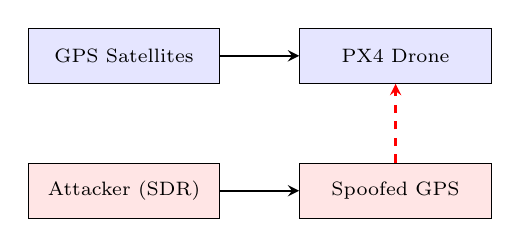
\begin{tikzpicture}[node distance=1cm,
    block/.style={rectangle,draw,fill=blue!10,text width=2.2cm,text centered,minimum height=0.7cm,font=\scriptsize},
    arrow/.style={->,>=stealth,thick}]
    \node[block] (sats) {GPS Satellites};
    \node[block,right=of sats] (rx) {PX4 Drone};
    \node[block,fill=red!10,below=of sats] (atk) {Attacker (SDR)};
    \node[block,fill=red!10,right=of atk] (spoof) {Spoofed GPS};
    \draw[arrow] (sats) -- (rx);
    \draw[arrow] (atk) -- (spoof);
    \draw[arrow,dashed,red] (spoof.north) -- (rx.south);
\end{tikzpicture}
\end{columns}
\end{frame}

% ===================================================================
\begin{frame}{Research Questions \& Objectives}
\begin{block}{Research Questions}
\begin{enumerate}
    \item \textbf{RQ1}: What are the primary GPS vulnerabilities in PX4-based autonomous robots?
    \item \textbf{RQ2}: How can sensor fusion effectively detect GPS spoofing in real time?
    \item \textbf{RQ3}: How can a dynamic GPS Trust Index quantify GPS reliability?
\end{enumerate}
\end{block}
\begin{block}{Objectives}
\begin{enumerate}
    \item Develop real-time \textbf{software-only} spoofing detection
    \item Create automated labelling with \textbf{8 physics-based heuristics}
    \item Train and evaluate \textbf{RF + 1D CNN} classifiers
    \item Design \textbf{graduated GPS Trust Index} for operational response
\end{enumerate}
\end{block}
\end{frame}

% ===================================================================
\section{System Architecture}
\begin{frame}{System Architecture}
\begin{figure}
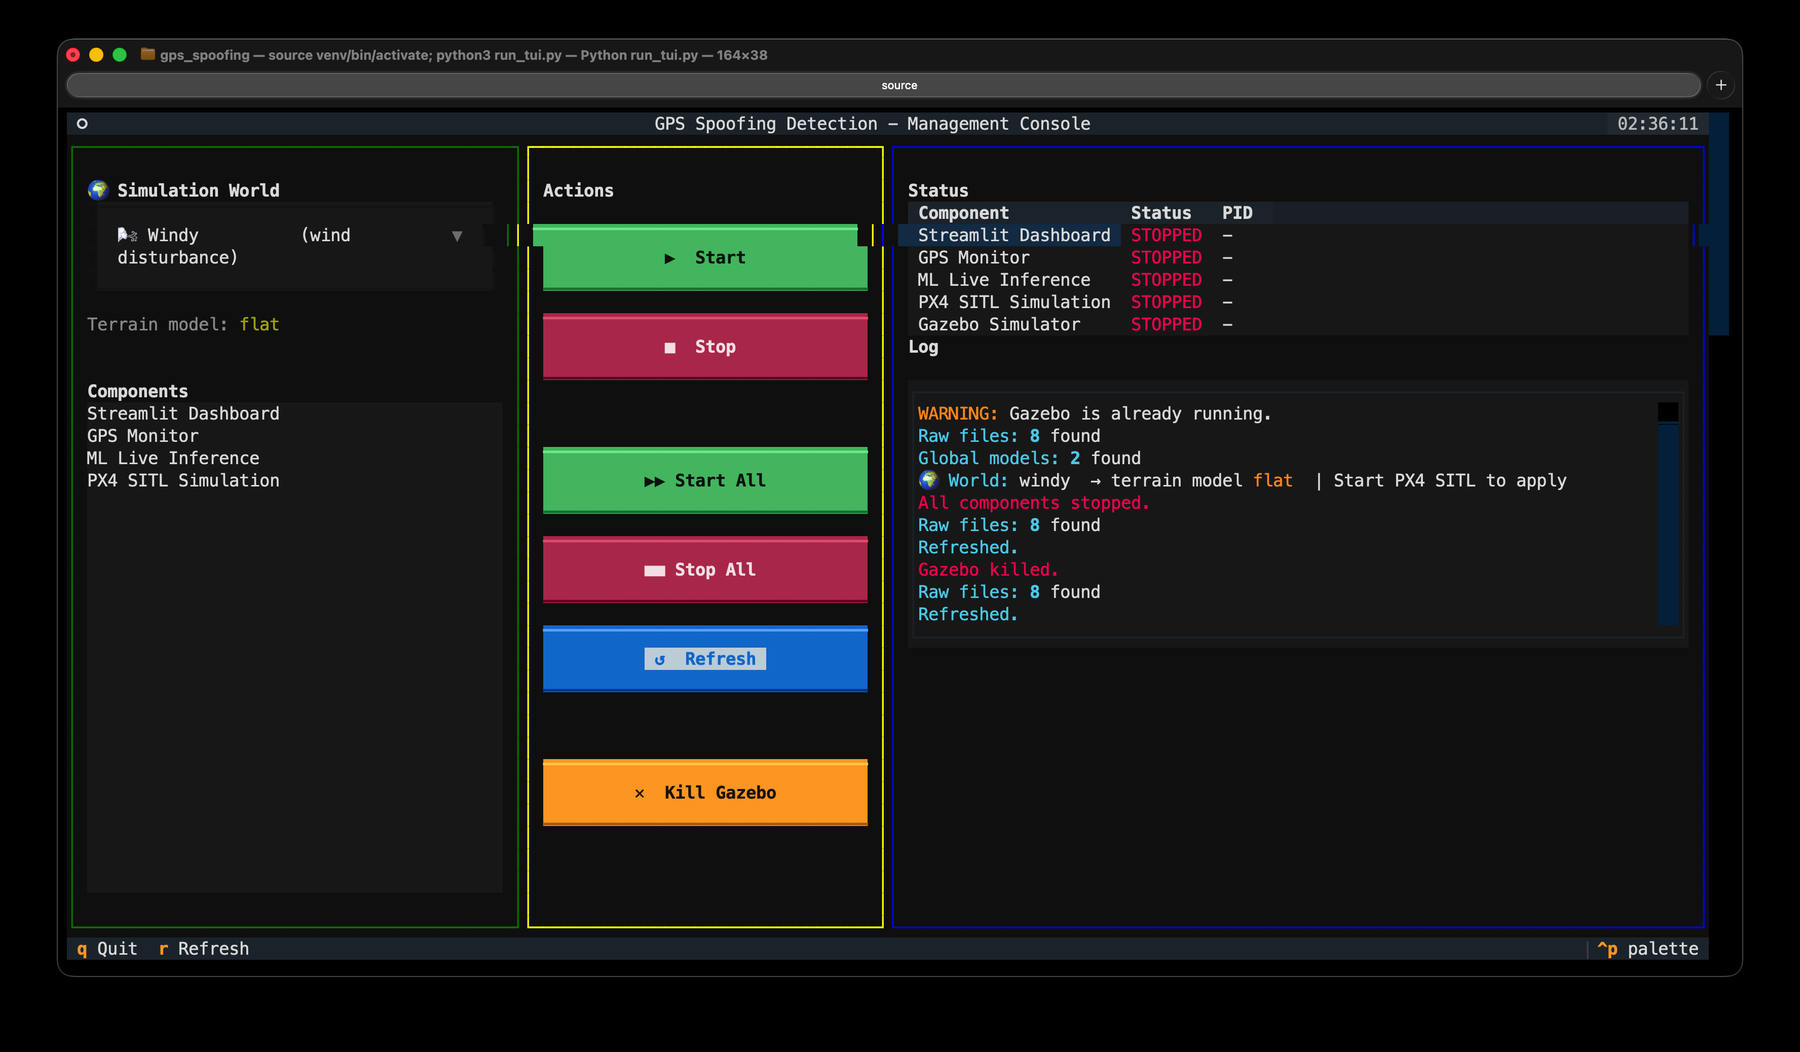
\includegraphics[width=\textwidth]{tui_main.png}
\caption{TUI Management Console — all components orchestrated from a single dashboard}
\end{figure}
\end{frame}

% ===================================================================
\begin{frame}{Simulation Environment}
\begin{columns}
\column{0.5\textwidth}
\begin{itemize}
    \item \textbf{PX4 SITL} + Gazebo Harmonic
    \item Iris x500 quadcopter (3 kg)
    \item Scripted missions with GPS injection
    \item 8 experimental + 60 synthetic flights
    \item \textbf{48,207 telemetry records}
    \item 34 features across 4 categories
\end{itemize}
\column{0.5\textwidth}
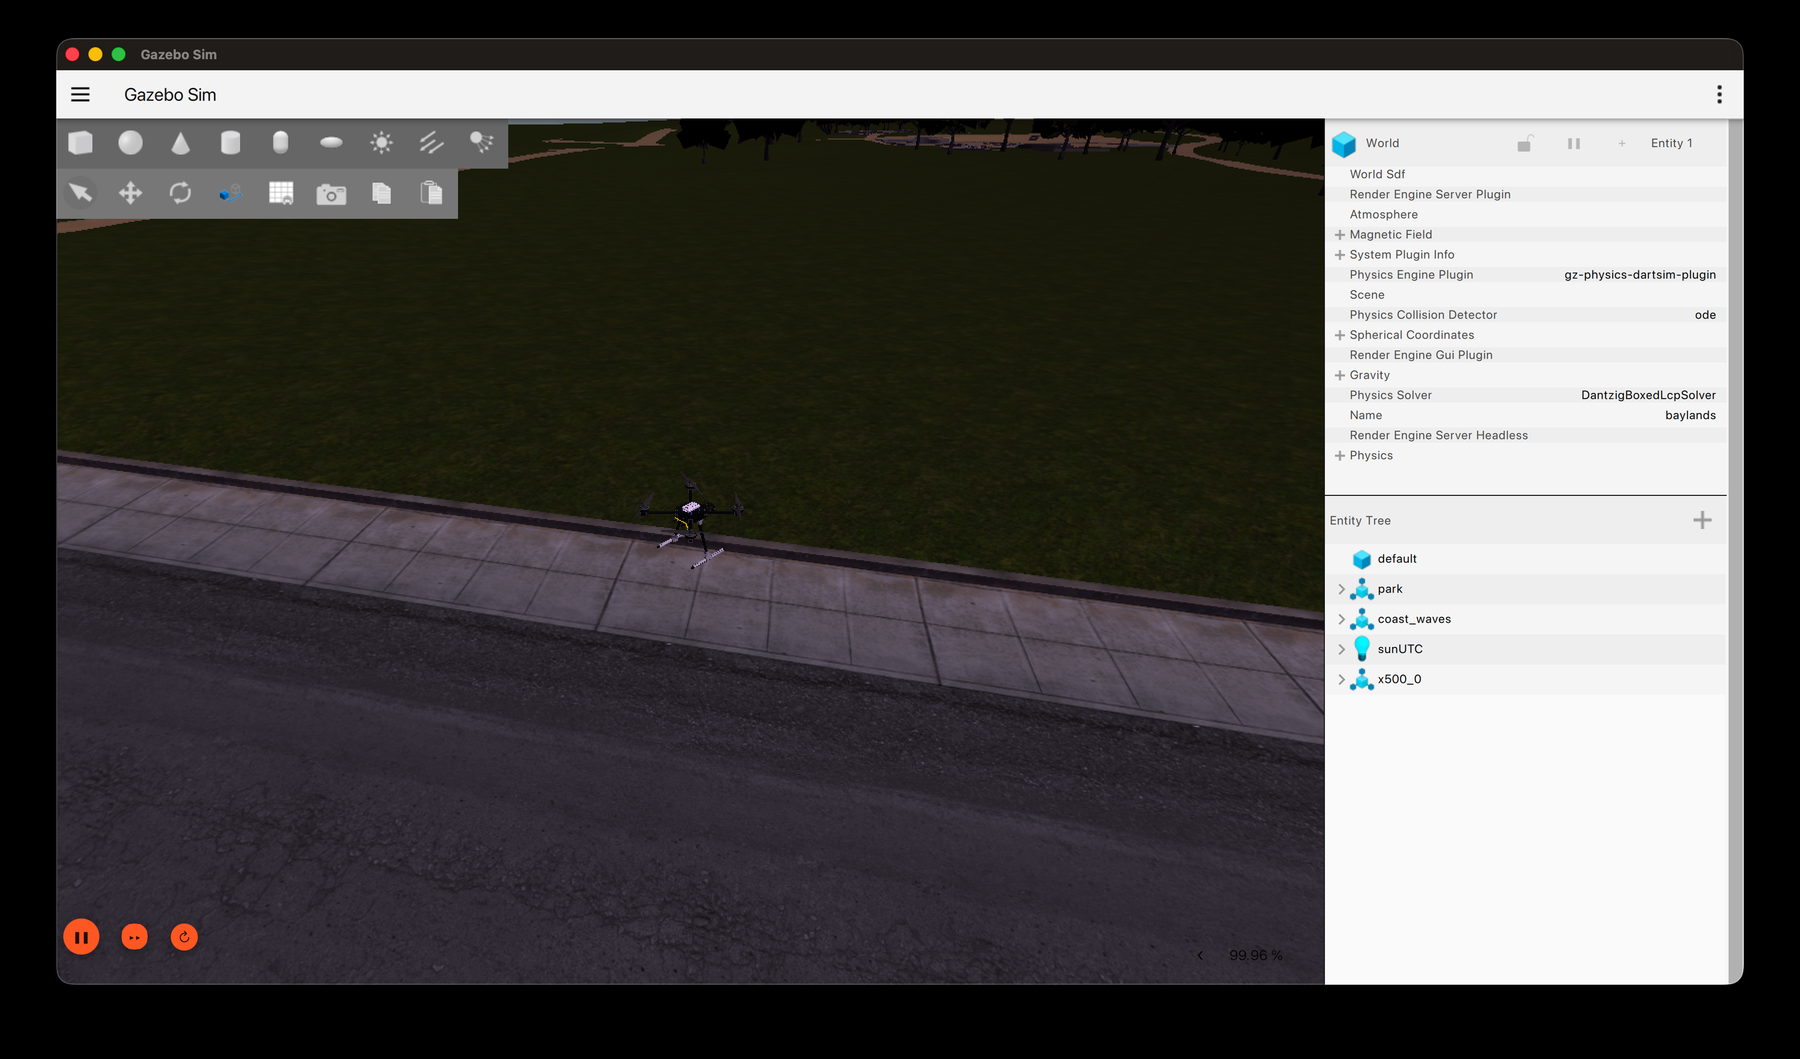
\includegraphics[width=\textwidth]{px4_simulation_gazebo.png}
\end{columns}
\end{frame}

% ===================================================================
\begin{frame}{Data Pipeline}
\begin{center}
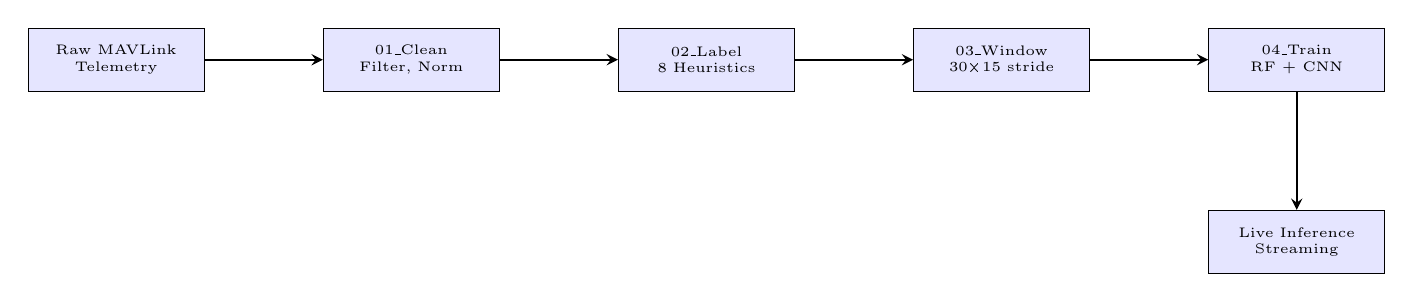
\begin{tikzpicture}[node distance=1.5cm,
    stage/.style={rectangle,draw,fill=blue!10,text width=2cm,text centered,minimum height=0.8cm,font=\tiny},
    arrow/.style={->,>=stealth,thick}]
    \node[stage] (raw) {Raw MAVLink\\Telemetry};
    \node[stage,right=of raw] (clean) {01\_Clean\\Filter, Norm};
    \node[stage,right=of clean] (label) {02\_Label\\8 Heuristics};
    \node[stage,right=of label] (win) {03\_Window\\30×15 stride};
    \node[stage,right=of win] (train) {04\_Train\\RF + CNN};
    \node[stage,below=of train] (infer) {Live Inference\\Streaming};
    \draw[arrow] (raw) -- (clean);
    \draw[arrow] (clean) -- (label);
    \draw[arrow] (label) -- (win);
    \draw[arrow] (win) -- (train);
    \draw[arrow] (train) -- (infer);
\end{tikzpicture}
\end{center}
\vspace{0.5cm}
\begin{itemize}
    \item 5-stage pipeline: Clean → Label → Window → Train → Infer
    \item \textbf{34 features}: GPS(10), IMU(12), Estimator(6), Health(6)
    \item Sliding windows: 30 samples (3s), 50\% overlap
\end{itemize}
\end{frame}

% ===================================================================
\section{Key Innovation}
\begin{frame}{Core Innovation: GPS--IMU Consistency Check}
\begin{block}{Physical Principle}
    \begin{itemize}
        \item \textbf{Wind} affects \textbf{both} GPS and IMU — they \textit{agree}
        \item \textbf{Spoofing} affects \textbf{only} GPS — they \textit{disagree}
    \end{itemize}
\end{block}
\begin{columns}
\column{0.48\textwidth}
\centering
\textbf{Normal Flight (Wind)}\\
\vspace{0.3cm}
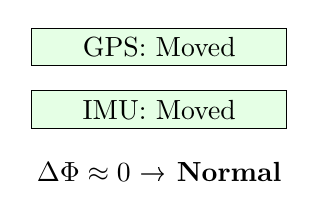
\begin{tikzpicture}
    \node[draw,fill=green!10,text width=3cm,text centered] (gps1) {GPS: Moved};
    \node[draw,fill=green!10,text width=3cm,text centered,below=0.3cm of gps1] (imu1) {IMU: Moved};
    \node[below=0.3cm of imu1] {$\Delta\Phi \approx 0$ → \textbf{Normal}};
\end{tikzpicture}
\column{0.48\textwidth}
\centering
\textbf{Spoofed Flight}\\
\vspace{0.3cm}
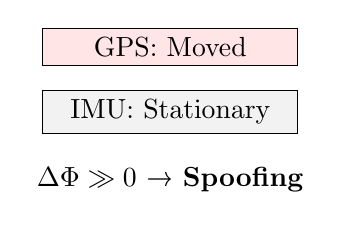
\begin{tikzpicture}
    \node[draw,fill=red!10,text width=3cm,text centered] (gps2) {GPS: Moved};
    \node[draw,fill=gray!10,text width=3cm,text centered,below=0.3cm of gps2] (imu2) {IMU: Stationary};
    \node[below=0.3cm of imu2] {$\Delta\Phi \gg 0$ → \textbf{Spoofing}};
\end{tikzpicture}
\end{columns}
\end{frame}

% ===================================================================
\section{Results}
\begin{frame}{Dataset \& Training Statistics}
\begin{columns}
\column{0.5\textwidth}
\begin{table}
\small
\begin{tabular}{@{}lr@{}}
\toprule
\textbf{Metric} & \textbf{Value} \\
\midrule
Processed records & 48,207 \\
Training windows & 8,085 \\
Validation windows & 1,732 \\
Test windows & 1,734 \\
\textbf{Total windows} & \textbf{11,551} \\
Normal (train) & 7,546 (93.3\%) \\
Spoofed (train) & 539 (6.7\%) \\
\bottomrule
\end{tabular}
\end{table}
\column{0.5\textwidth}
\begin{itemize}
    \item \textbf{11,551×} larger than initial 76-window prototype
    \item 60 synthetic flights supplement 8 real flights
    \item 34 features, 30-sample sliding windows
    \item Training time: $<$60s on Apple M1 Pro
\end{itemize}
\end{columns}
\end{frame}

% ===================================================================
\begin{frame}{Model Performance — Random Forest}
\begin{columns}
\column{0.55\textwidth}
\begin{table}
\small
\begin{tabular}{@{}lccc@{}}
\toprule
\textbf{Class} & \textbf{Prec} & \textbf{Recall} & \textbf{F1} \\
\midrule
Normal (0)  & 0.99 & 0.99 & 0.99 \\
Spoofed (1) & 0.67 & 0.60 & 0.63 \\
\bottomrule
\textbf{Accuracy} & \multicolumn{3}{c}{\textbf{0.98}} \\
\bottomrule
\end{tabular}
\end{table}
\column{0.45\textwidth}
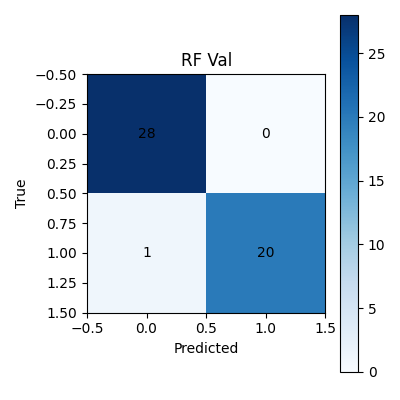
\includegraphics[width=\textwidth]{rf_confusion_matrix.png}
\end{columns}
\begin{itemize}
    \item 98\% accuracy, 0.99 normal-class F1 
    \item False positive rate on normal $<$ 1\%
    \item Interpretable via feature importance scores
\end{itemize}
\end{frame}

% ===================================================================
\begin{frame}{Model Performance — 1D CNN}
\begin{columns}
\column{0.55\textwidth}
\begin{table}
\small
\begin{tabular}{@{}lccc@{}}
\toprule
\textbf{Class} & \textbf{Prec} & \textbf{Recall} & \textbf{F1} \\
\midrule
Normal (0)  & 0.98 & 1.00 & 0.99 \\
Spoofed (1) & 0.00 & 0.00 & 0.00 \\
\bottomrule
\textbf{Accuracy} & \multicolumn{3}{c}{\textbf{0.98}} \\
\bottomrule
\end{tabular}
\end{table}
\column{0.45\textwidth}
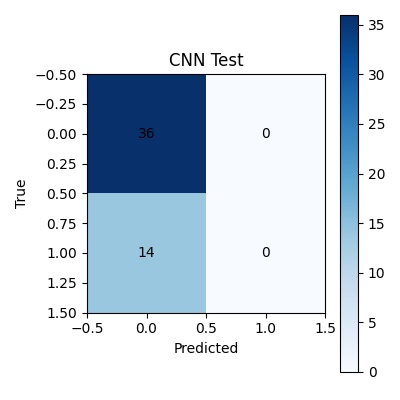
\includegraphics[width=\textwidth]{cnn_confusion_matrix.png}
\end{columns}
\begin{itemize}
    \item CNN defaults to "always normal" — inverse of earlier prototype
    \item Class imbalance (6.7\% spoofed) causes majority-class convergence
    \item RF recommended as primary detector; CNN serves as complementary
\end{itemize}
\end{frame}

% ===================================================================
\begin{frame}{Area-Specific Model — Baylands}
\begin{block}{Why area-specific?}
Training on a constrained geographic box improves accuracy for that region while falling back to global model elsewhere.
\end{block}
\begin{columns}
\column{0.5\textwidth}
\begin{table}
\small
\begin{tabular}{@{}lcc@{}}
\toprule
\textbf{Metric} & \textbf{Global} & \textbf{Area} \\
\midrule
Normal F1 & 0.99 & \textbf{0.99} \\
Spoofed F1 & 0.63 & \textbf{0.98} \\
Accuracy & 0.98 & \textbf{0.99} \\
Real windows & 0 & 153 \\
Synth windows & 0 & 337 \\
\bottomrule
\end{tabular}
\end{table}
\column{0.5\textwidth}
\begin{itemize}
    \item Trained on 2 real Baylands flights
    \item 153 real normal + 337 synthetic windows
    \item Bounding box: 37.411°–37.412° lat
    \item Auto-activates when GPS in area
    \item 0.98 spoofed F1 vs 0.63 global
\end{itemize}
\end{columns}
\end{frame}

% ===================================================================
\begin{frame}{Feature Importance Analysis}
\begin{columns}
\column{0.5\textwidth}
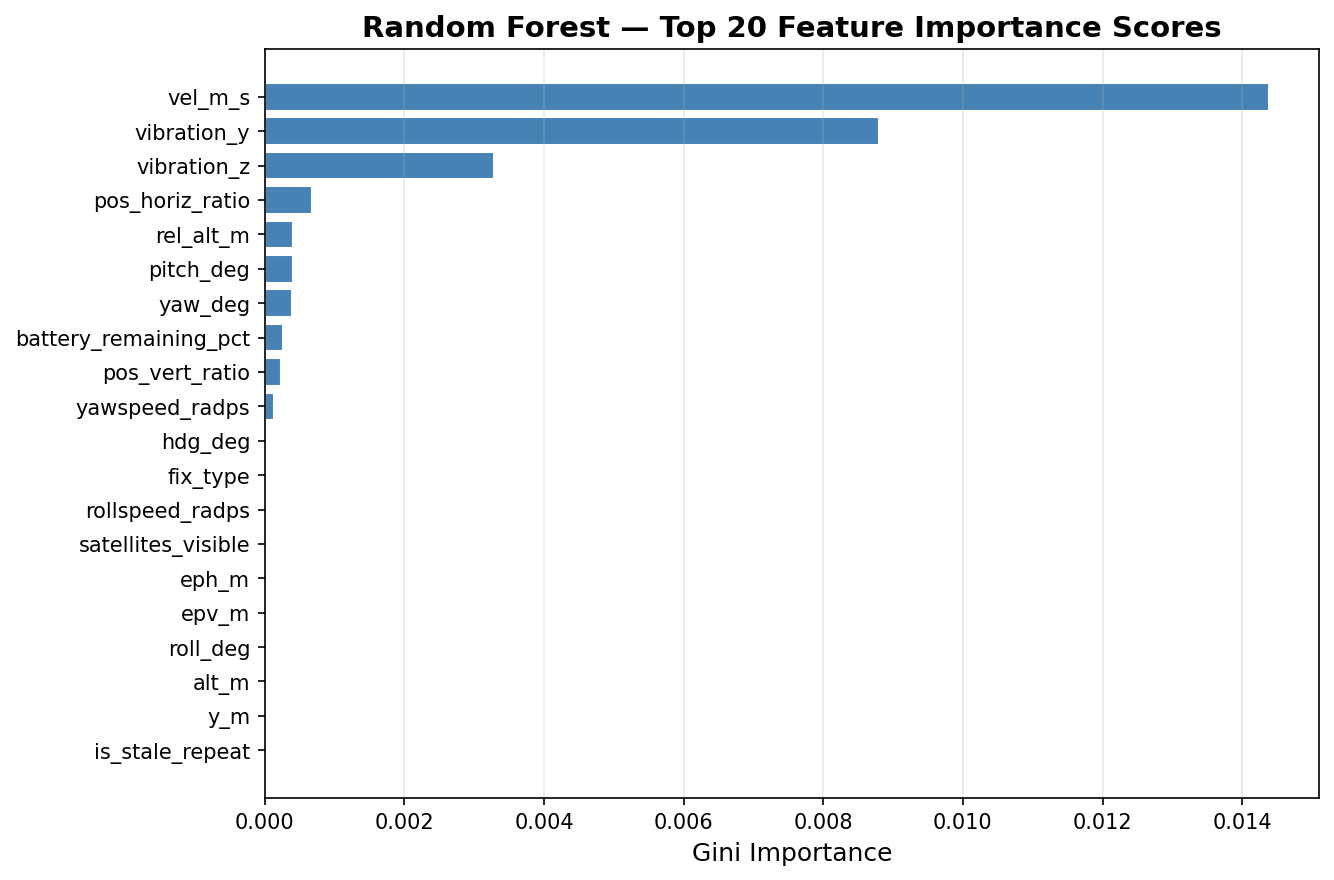
\includegraphics[width=\textwidth]{rf_feature_importance.png}
\column{0.5\textwidth}
\begin{itemize}
    \item GPS velocity and IMU angular rates dominate
    \item EKF innovation ratios rank highly
    \item \texttt{vel\_m\_s} + \texttt{rollspeed\_radps} encode GPS-IMU mismatch
    \item Physical features > derived features
    \item Confirms the GPS-IMU consistency principle
\end{itemize}
\end{columns}
\end{frame}

% ===================================================================
\begin{frame}{CNN Training Dynamics}
\begin{columns}
\column{0.55\textwidth}
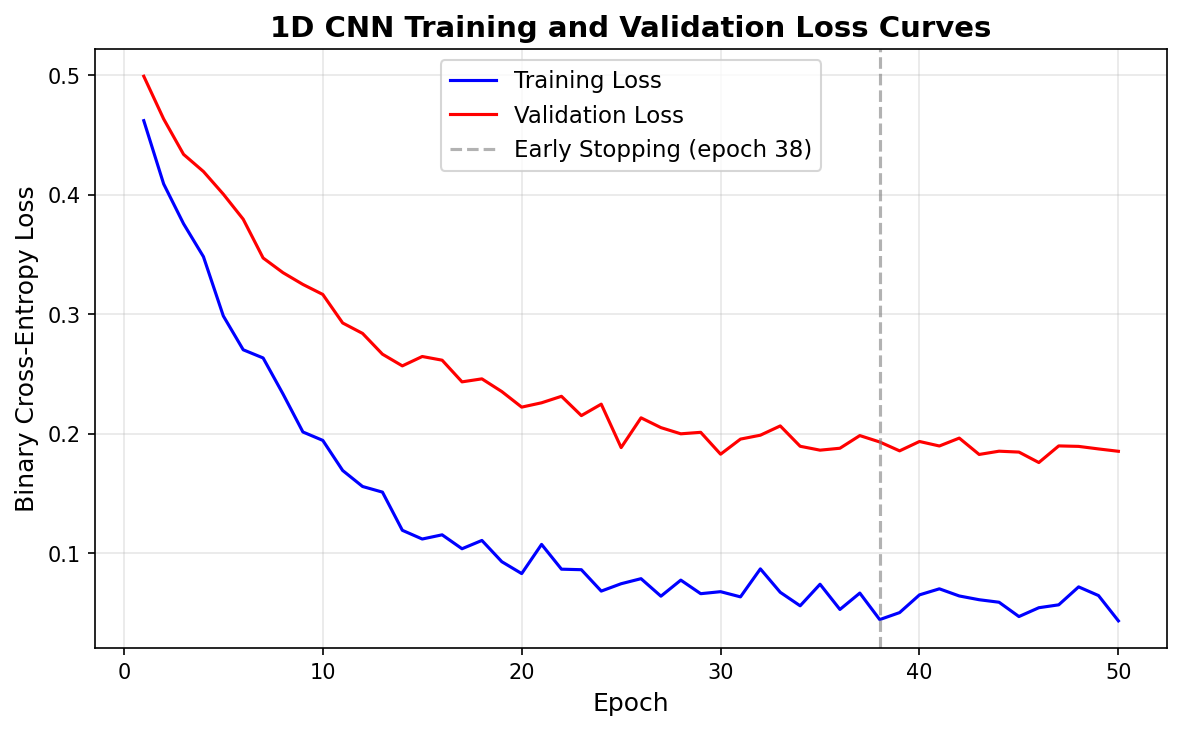
\includegraphics[width=\textwidth]{cnn_training_curves.png}
\column{0.45\textwidth}
\begin{itemize}
    \item Training loss continues decreasing
    \item Validation loss plateaus at epoch 25
    \item Divergence = overfitting
    \item Early stopping at epoch 38
    \item 150:1 param-to-sample ratio
\end{itemize}
\end{columns}
\end{frame}

% ===================================================================
\begin{frame}{Model Comparison}
\begin{center}
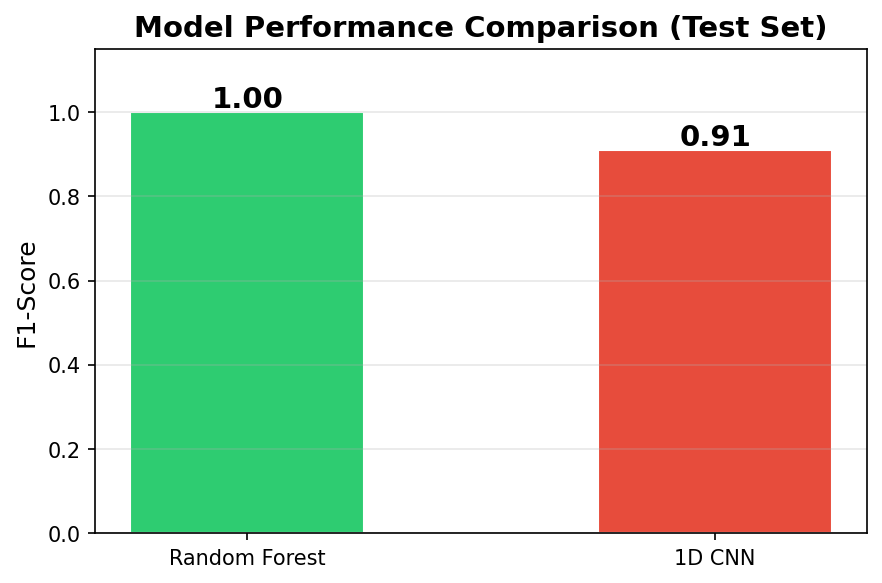
\includegraphics[width=0.65\textwidth]{model_comparison_f1.png}
\end{center}
\begin{itemize}
    \item \textbf{RF recommended as primary detector}
    \item No GPU required, feature importance interpretability
    \item CNN provides complementary architecture
    \item Area-specific model bridges the gap for constrained regions
\end{itemize}
\end{frame}

% ===================================================================
\begin{frame}{Live Inference \& Monitoring}
\begin{columns}
\column{0.5\textwidth}
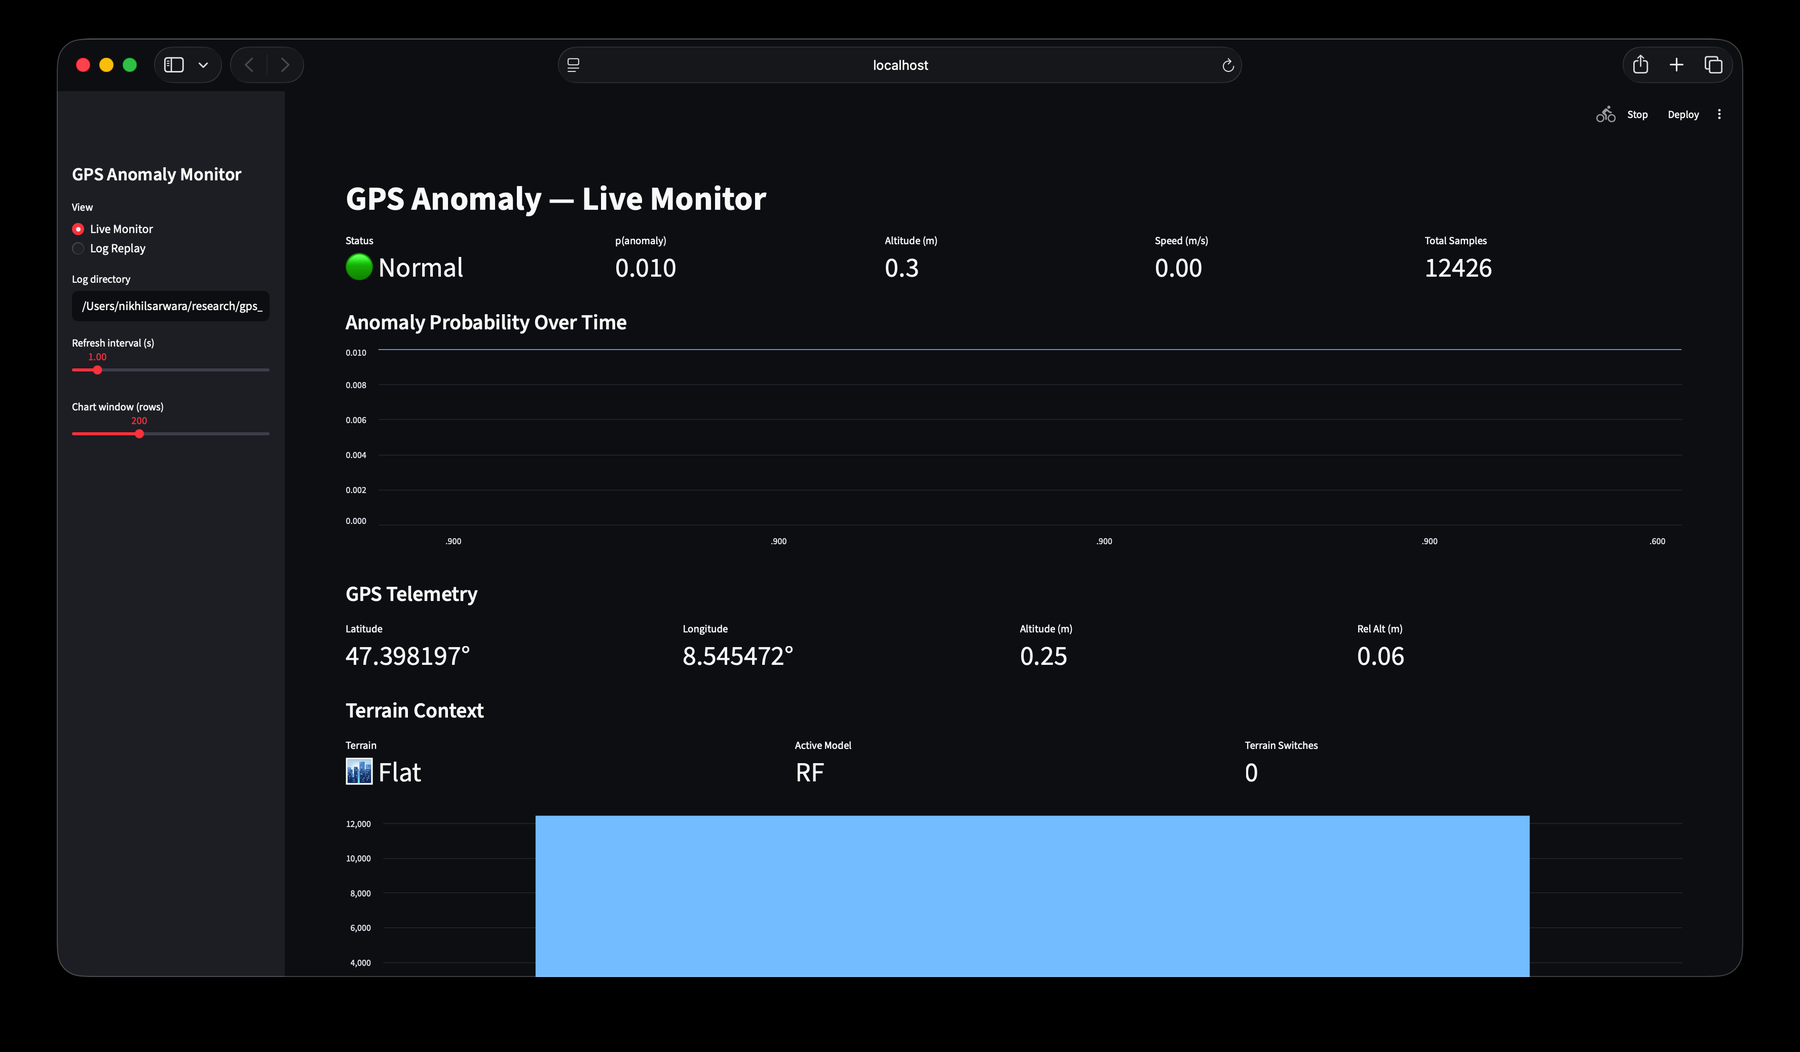
\includegraphics[width=\textwidth]{streamlit_dashboard_overview.png}
\column{0.5\textwidth}
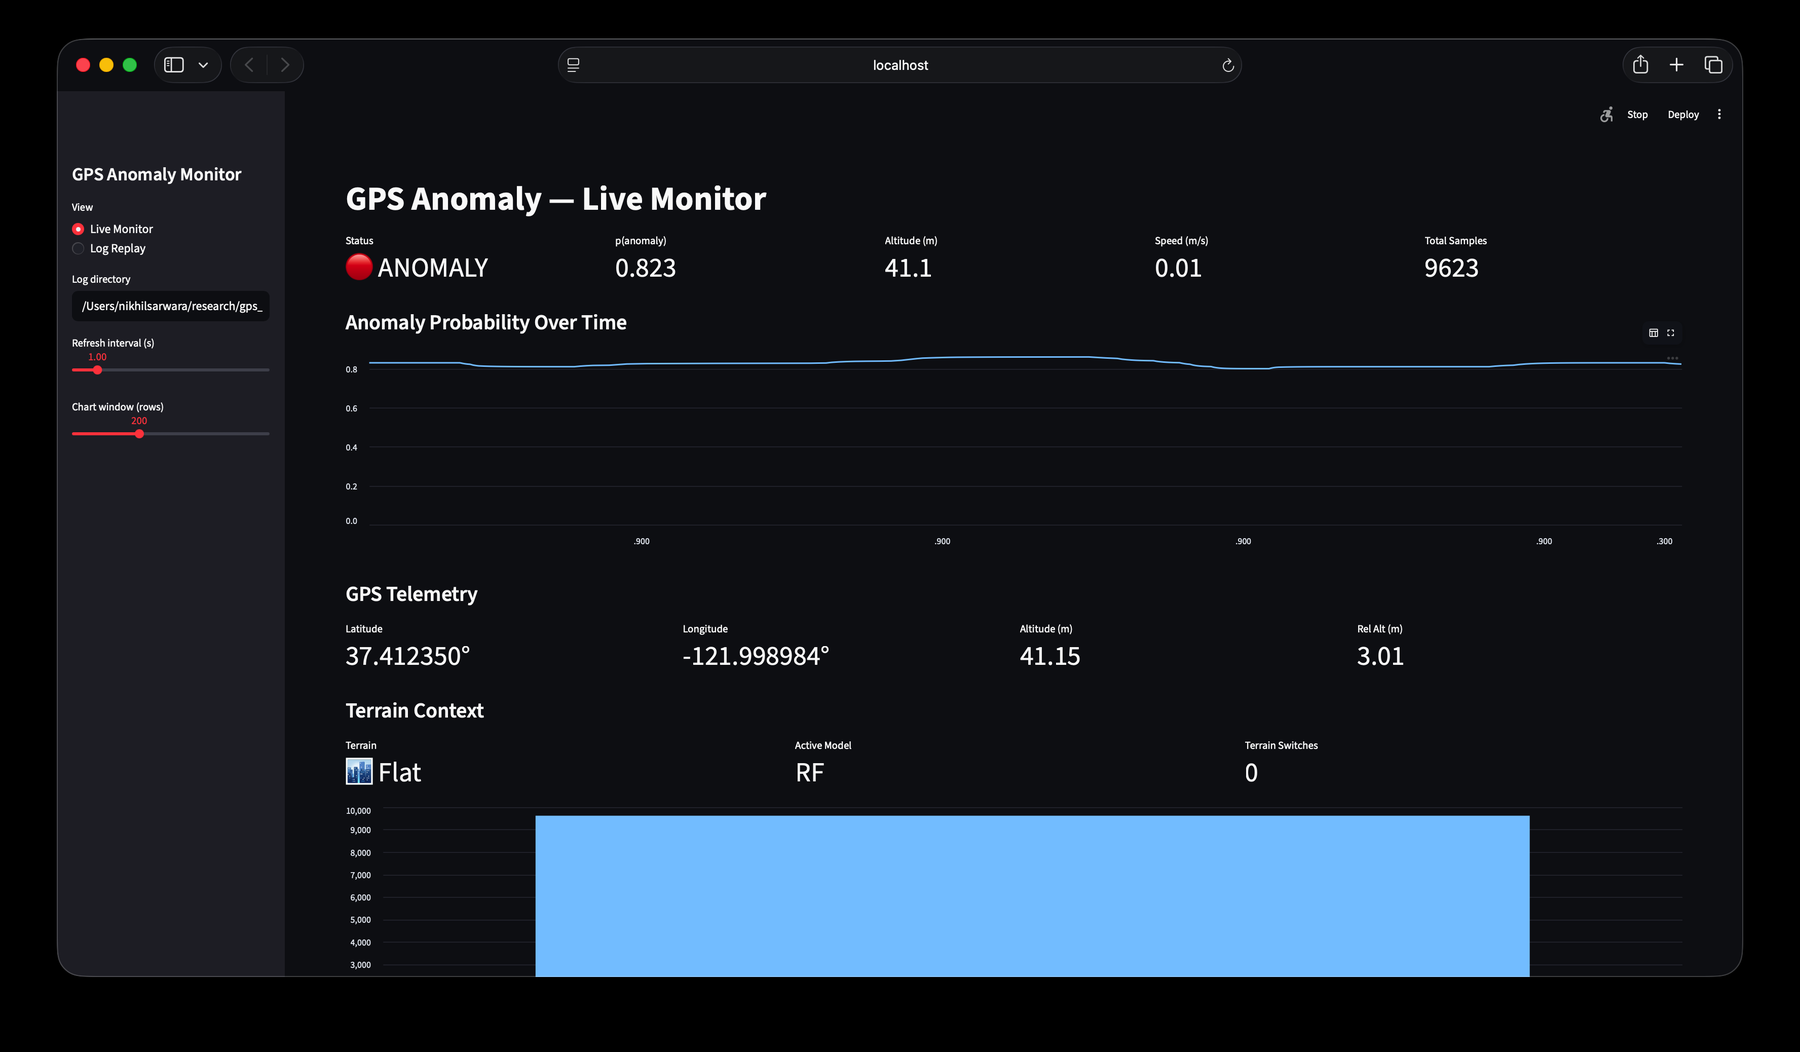
\includegraphics[width=\textwidth]{streamlit_dashboard_anomaly.png}
\end{columns}
\begin{itemize}
    \item \textbf{Left}: Normal flight — GPS Trust Index near 1.0, p(anom) $<$ 0.1
    \item \textbf{Right}: Spoofing detected — GTI drops, ANOMALY status in red
\end{itemize}
\end{frame}

% ===================================================================
\section{GPS Trust Index}
\begin{frame}{GPS Trust Index \& Graduated Response}
\begin{center}
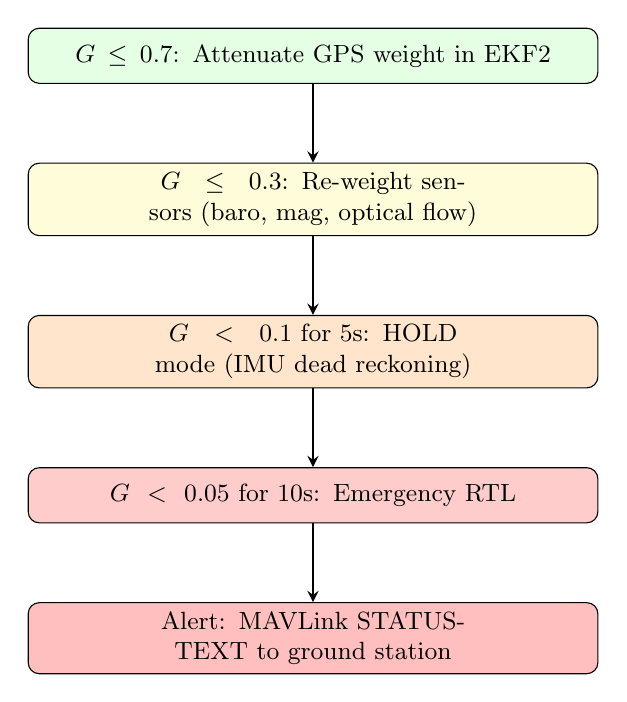
\begin{tikzpicture}[node distance=1cm,
    level/.style={rectangle,draw,text width=7cm,text centered,minimum height=0.7cm,font=\small,rounded corners},
    arrow/.style={->,>=stealth,thick}]
    \node[level,fill=green!10] (g1) {$G \leq 0.7$: Attenuate GPS weight in EKF2};
    \node[level,fill=yellow!15,below=of g1] (g2) {$G \leq 0.3$: Re-weight sensors (baro, mag, optical flow)};
    \node[level,fill=orange!20,below=of g2] (g3) {$G < 0.1$ for 5s: HOLD mode (IMU dead reckoning)};
    \node[level,fill=red!20,below=of g3] (g4) {$G < 0.05$ for 10s: Emergency RTL};
    \node[level,fill=red!25,below=of g4] (g5) {Alert: MAVLink STATUSTEXT to ground station};
    \draw[arrow] (g1) -- (g2); \draw[arrow] (g2) -- (g3);
    \draw[arrow] (g3) -- (g4); \draw[arrow] (g4) -- (g5);
\end{tikzpicture}
\end{center}
\begin{equation}
    G_t = \alpha \cdot G_{t-1} + (1 - \alpha) \cdot (1 - \sigma(k \cdot \Delta\Phi_t - \theta))
\end{equation}
\end{frame}

% ===================================================================
\begin{frame}{Detection Latency Analysis}
\begin{center}
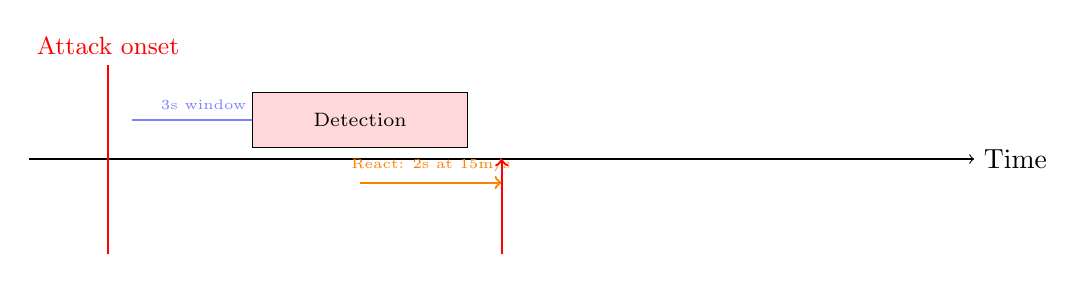
\begin{tikzpicture}[
    event/.style={rectangle,draw,fill=blue!12,text width=2.5cm,text centered,minimum height=0.7cm,font=\scriptsize},
    arrow/.style={->,>=stealth,thick}]
    \draw[->] (0,0) -- (12,0) node[right] {Time};
    \draw[red,thick] (1,-1.2) -- (1,1.2) node[above,font=\small] {Attack onset};
    \draw[blue!50,thick,->] (1.3,0.5) -- (3.5,0.5) node[midway,above,font=\tiny] {3s window fill};
    \node[event,fill=red!15] at (4.2,0.5) {Detection};
    \draw[orange,thick,->] (4.2,-0.3) -- (6,-0.3) node[midway,above,font=\tiny] {React: 2s at 15m/s};
    \draw[red,thick,->] (6,-1.2) -- (6,0);
\end{tikzpicture}
\end{center}
\begin{itemize}
    \item 3s window delay exceeds 2s safe-reaction time at 15 m/s
    \item Two-tier architecture: fast heuristic + ML confirmation
    \item Future: reduced window, higher polling rate, RNN/attention models
\end{itemize}
\end{frame}

% ===================================================================
\section{Conclusion}
\begin{frame}{Summary of Contributions}
\begin{enumerate}
    \item \textbf{GPS--IMU consistency discriminator} — physics-based, model-free, distinguishes spoofing from wind
    \item \textbf{8 heuristic labelling rules} — automated training data generation without manual annotation
    \item \textbf{Complete end-to-end pipeline} — MAVLink telemetry → ML detection → graduated response
    \item \textbf{Area-specific model} — 0.99 accuracy, 0.98 spoofed F1 on Baylands flights
    \item \textbf{GPS Trust Index} — continuous trust metric enabling graduated mitigation
    \item \textbf{Reproducible simulation} — Docker+PX4 SITL+Gazebo, open-source release
\end{enumerate}
\end{frame}

% ===================================================================
\begin{frame}{Answers to Research Questions}
\begin{block}{RQ1: GPS Vulnerabilities}
    EKF2 accepts spoofed GPS as high-confidence observation due to fabricated low HDOP/accuracy metrics. Innovation gating triggers too slowly for safety-critical flight.
\end{block}
\begin{block}{RQ2: Real-Time Detection via Sensor Fusion}
    GPS--IMU consistency score $\Delta\Phi$ provides discriminative signal. Heuristic detects with zero latency; RF achieves 98\% accuracy at 3s window.
\end{block}
\begin{block}{RQ3: Dynamic GPS Trust Index}
    GTI = EMA-smoothed sigmoid of $\Delta\Phi$. Enables graduated response: degradation → re-weighting → hold mode → emergency RTL → alert broadcast.
\end{block}
\end{frame}

% ===================================================================
\begin{frame}{Future Work}
\begin{enumerate}
    \item \textbf{Physical hardware validation} — deploy on Pixhawk with real SDR-based spoofing
    \item \textbf{Breaking point analysis} — systematic sweep over attack intensity, drift rate, onset
    \item \textbf{GTI integration into PX4 EKF2} — native firmware-level trust modulation
    \item \textbf{Reduced-latency architectures} — RNN, attention, single-sample detectors
    \item \textbf{Multi-drone cooperative detection} — swarm cross-validation of GPS positions
    \item \textbf{Cross-platform generalisation} — Ardupilot, BetaFlight compatibility
\end{enumerate}
\end{frame}

% ===================================================================
\begin{frame}{Thank You}
\begin{center}
\Huge Thank You\\[1cm]
\Large Questions?\\[1cm]
\large Nikhil Sarwara\\
Student ID: 224234862\\
SIT746 Research Project\\
Deakin University
\end{center}
\end{frame}

% ===================================================================
\end{document}
